\chapter{Metodologia} \label{metodologia}

Neste capítulo, apresentaremos as ferramentas que adotamos para a análise de sentimentos dos dados obtidos nos \textit{corpus} textuais; tecnicas de \textit{web scraping} e \textit{text minning}; critérios de frequência de distribuições empíricas de probabilidades; e a análise de sentimento. Para esse efeito, dividimos esse capítulo em três partes: a primeira contém as ferramentas de \textit{web scraping} e \textit{text minning}; a segunda o critério de divergência de Kullback-Leibler; e por fim, será feito uma descrição de como funciona a análise de sentimento por meio de um dicionário léxico. 

\section{Web Scraping}

\textit{Web scraping} (ou raspagem de dados) pode ser definida como a tecnica de extração e coleta de dados a partir de um ambiente web, possibilitando uma automatização de obtenção de dados como um todo. Desta forma, a partir de algorítimos voltados para a automatização da coleta é possível a obtenção de grandes volumes de dados - feito que manualmente poderia ser \textit{extremamente} custoso.

Podemos demonstrar o processo por meio de um circuito (figura \ref{fig:webscraping}) iterativo. Dado o momento em que podemos coletar um dado específico de um site, por exemplo uma classe específica de um ambiente HTML, é possível a generalização na coleta de dados que acabam por seguir o mesmo padrão deste - dado uma conexão com o servidor deste site.  

\begin{figure}[!h]
    \centering
    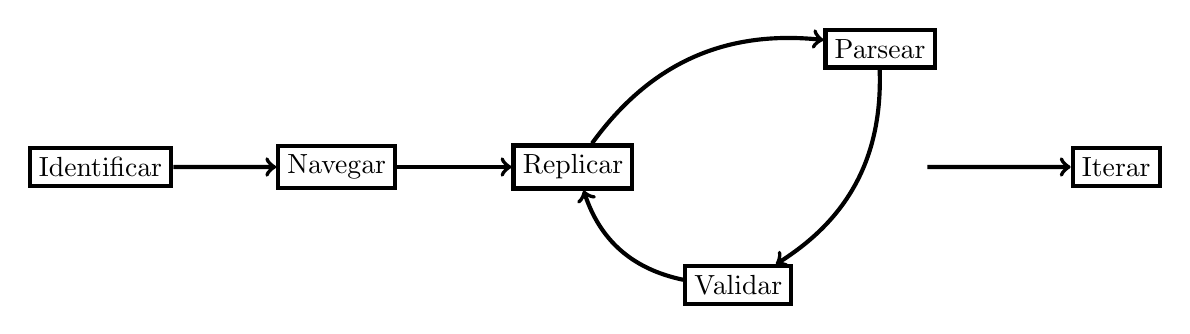
\begin{tikzpicture}[scale = 3, line width = 1.5pt]
\draw
    (1,1) node[ draw](a1){Identificar}
    (2,1) node[ draw](a2){Navegar}
    (3,1) node[ draw](a3){Replicar}
    (4.3,1.5) node[ draw](a4){Parsear}
    (3.7,0.5) node[draw](a5){Validar}
    (5.3,1) node[ draw, line width = 1.5](a6){Iterar};
    
    \draw [->] (a1) -- (a2) node[midway,below] {};
    \draw [->] (a2) -- (a3) node[midway,above] {};
    \draw[->] (4.5,1) -- (a6);
    
    \path[->] (a5) edge [bend left = 30] node[left, red] {} (a3);
    \path[->] (a3) edge [bend left = 30] node[left, red] {} (a4);
    \path[->] (a4) edge [bend left = 30] node[left, red] {} (a5);
                                                                                                                                                                                                                                                                                                                                                                                                                                                                                                                                            
\end{tikzpicture}

    \caption{Fluxo de funcionamento de um web scraping}
    \label{fig:webscraping}
\end{figure}

A possibilidade da reprodução de algorítmos por meio de \textit{web scraping} nos permite - por vezes - realizarmos coletas volumosas de dados da internet, como por exemplo, dados econômicos estruturados e não-estruturados. 

\subsection{O Fluxo de Funcionamento do \textit{web scraping}}

Utilizando termos mais técnicos, o funcionamento do \textit{web scraping} é baseado num fluxo partindo da identificação dos dados a serem coletados; a \textit{navegação} web; um fluxo interativo (replicação, \textit{parseamento} e validação); e finalmente a Iteração dos dados.\cite{web2019}

O primeiro passo, quando nos referimos a identificação, é definirmos o que queremos coletar. No presente trabalho, o foco se restringe as atas do COPOM (minutes), disponíveis em inglês. Definem-se as páginas no site do Banco Central, e a partir delas, busca-se as informações necessárias para a coleta.  \cite{costa2016ensaios}. Tendo identificado nosso objetivo, foi feita uma seleção das atas necessárias para o presente trabalho. Como o escopo do estudo foram as atas do ano de 2003 ao ano de 2018, por meio de um algorítimo\footnote{http://selectorgadget.com/} definimos onde deveríamos trabalhar. A replicação dos dados ocorre por meio de um script no software R, no qual realizamos todo o processo anterior, bem como o download das atas. A iteratividade realizada nos permite baixar todas as atas em pdf, bem como armazená-las para o estudo posterior.


\subsection{Utilidades mais comuns do \textit{web scraping}}
O \textit{web scraping} cada vez mais vem sendo utilizado no mundo empresarial e em políticas públicas. A partir deste, é possível monitorar atividades em tempo real, bem como variações de preços ou acontecimentos políticos de forma automatica.

De forma mais generalizada, exemplos de aplicações do \textit{web scraping} podem ser dados como: 1 - \textbf{área comercial e de vendas}, visto que é possível qualificar base de dados de maneira automática bem como adicionar informações às mesmas - como informações de clientes, ou algo que possa interessar; 2 - \textbf{monitorar preços de concorrência}, manter listado e atualizado a preços reais variações de preços, bem como lista de vendas de setores específicos; 3 - \textbf{\textit{marketing} e investigação de mercado}, investigar compradores, tendências, monitorar marcas. Neste ponto, o \textit{web scraping} pode ser utilizado para - desde a monitoração de fóruns \textit{onlines} até - investigações de tendências em redes sociais \cite{web2019utilidade}.

\section{A Divergencia de Kullback-Liebler}

Como partes das ferramentas estatísticas na análise de discrepâncias ou semelhanças entre variáveis aleatórias, foi proposto a divergência de Kullback-Liebler (K-L). É importante salientar que esta função é base na construção do critério de Akaike para escolhas de modelos - critério muito utilizado na esfera econométrica \cite{wooldridge2006introduccao, gujarati2011econometria}.

\subsection{A Informação de Kullback-Liebler ou Entropia Relativa}

Sejam $f$ e $g$ distribuições de probabilidades simples. A informação de K-L, para o caso contínuo, pode ser dada por: 
\begin{align*}
I(f, g) = \int f(x)\log\left(\frac{f(x)}{g(x|\theta)}\right) \quad dx,
\end{align*}

onde $\log$ representa o logarítmo natural. A notação $I(f, g)$ representa `` a informação perdida quando $g$ é usado para aproximar $f$''. Dessa forma, $I(f, g)$ é a distância de $g$ para $f$. Uma interpretação da distância de K-L é em relação a uma medida de ineficiência: dado a distribuição $g$ quando a distribuição $f$ é verdadeira.

Para o caso de uma distribuição discreta, como Poisson, Binomial, ou Multinomial, teremos:
\begin{align*}
I(f, g) = \sum_{i=1}^{k} p_{i} \cdot \log\left( \frac{p_i}{\pi_i}\right),
\end{align*}

Nesse caso existem $k$ resultados possíveis. A verdadeira probabilidade do \textit{inésimo} termo é dada por $p_i$ enquanto $\pi_1, \dots, \pi_k$ constituem a distribuição de probabilidades aproximadas. Neste caso, teríamos: $0 < p_i < 1$, $0 < \pi < 1$ e desta forma: $\sum p_i = \sum \pi_i = 1$. Assim, $f$ e $g$ corresponderiam a $p_i$ e $\pi_i$ respectivamente \cite[p. 51]{burnham2002practical}.

Nesse caso, sendo as distribuições discretas iguais, teríamos $I(f,g) = 0 \iff p_i = \pi_i$. A medida de K-L, contextualizada como uma distância entre dois modelos - isso é, a discrepância entre eles.

\subsection{Exemplo 1}

Podemos ilustrar a distância de K-L ($I(f, g)$) simulando distribuições. Seja $f$ uma distribuição gamma com dois parâmetros ($\alpha = 4, \beta = 4$). Consideraremos, então, 4 distribuições (Tabela \ref{ref:tabeladist}) $g_i$, cada uma com 2 parâmetros: distribuição Weibull; lognormal; gaussiana inversa; e F de Fisher-Snedecor. A questão colocada é: ``qual dessas distribuições é a \textit{mais próxima} de $f$?'' \cite[p. 54]{burnham2002practical}

\begin{table}[!h]
\centering
\caption{Distribuições para comparação}
\begin{tabular}{lllc}
\hline
      & Modelo Aproximado                                            & $I(f, g_i)$ & Ordem \\ \hline
$g_1$ & Distribuição Weibull ($\alpha = 2, \beta = 20$)              & 0.046189    & 1     \\
$g_2$ & Distribuição Lognormal ($\theta = 2, \sigma^2 = 2$)          & 0.672316    & 2     \\
$g_3$ & Gaussiana Inversa ($\alpha = 16, \beta = 64$)                & 0.059960    & 3     \\
$g_4$ & Distribuição F de Fisher-Snedecor ($\alpha = 4, \beta = 10$) & 5.745504    & 4     \\ \hline
\end{tabular}
\label{ref:tabeladist}
\end{table}

de acordo com a tabela, a distribuição simulada que mais se aproxima da gamma - dado os parâmetros - é a distribuição de Weilbul, seguido pela gaussiana inversa.
\begin{figure}[!h]
    \centering
    \caption{Gráficos de gamma comparado às distribuições}
    \includegraphics[width=\textwidth, height=10cm]{capitulos/figures/graf_gamma_ggplot.pdf}
    \label{fig:my_label}
\end{figure}

\subsection{Exemplo 2}

Neste exemplo, desenvolvemos a informação de K-L e é feita uma ilustração gráfica do comportamento da entropia relativa em relação às variações nos parâmetros. 

\subsubsection{Modelos Normais}
\label{normal}

Supondo duas distribuições $g$ e $f$ normais $N(\Theta, \tau^2)$ e $N(\mu, \sigma^2)$ respectivamente. Se $E_G$ é a esperança referente a $g$ e $X$ é uma variável aleatória que segue $N(\mu, \sigma^2)$, temos \cite[p. 32]{konishi2008information} :
\begin{align*}
    E_G[(X - \mu)^2] &= E_G[(X - \Theta)^2 + 2(X - \Theta)(\Theta - \mu) + (\Theta - \mu)^2]\\
                     &= \tau^2 + (\Theta - \mu)^2
\end{align*}
então, para uma distribuição normal $f(x) = (2\pi\sigma^2)^{-\frac{1}{2}}\exp\{-(x - \mu)^2 / (2\sigma^2)\}$, temos:
\begin{align*}
    E_G[\log f(X)] &= E_G\left[\frac{1}{2}\log(2\pi\sigma^2)-\frac{(X-\mu)^2}{2\sigma^2}\right]\\
                   &= -\frac{1}{2}\log(2\pi\sigma^2) - \frac{\tau^2 + (\Theta - \mu)^2}{2\sigma^2}
\end{align*}
e, particular, se considerarmos $\mu = \Theta$ e $\sigma^2 = \tau^2$ nessa expressão, teremos:
\begin{align*}
    E_G[\log g(x)] = -\frac{1}{2}\log(2\pi\tau^2) - \frac{1}{2}
\end{align*}
assim, a distância de K-L de $f$ em relação a $g$ é dada por:
\begin{align*}
    I(g,f) &= E_G[\log g(X)] - E_G[\log f(X)]\\
           &= \frac{1}{2}\left\{\log\frac{\sigma^2}{\tau^2} + \frac{\tau^2 + (\Theta - \mu)^2}{\sigma^2} - 1 \right\}
\end{align*}

\noindent
a Figura \ref{fig:normal}, apresenta a variação de $I(f,g)$ dado que $\sigma^2 = 1$ e $\mu = 0$. $y$ representa $\tau$ e $x$ representa $\Theta$, da última equação. Na escala, os valores aproximados para a divergência de K-L.

\begin{figure}[!h]
    \centering
    \caption{Comparações de $I(f,g)$ quando $\Theta$ e $tau$ variam (\ref{normal}), assumindo uma normal padrão ($N(0, 1)$)}
    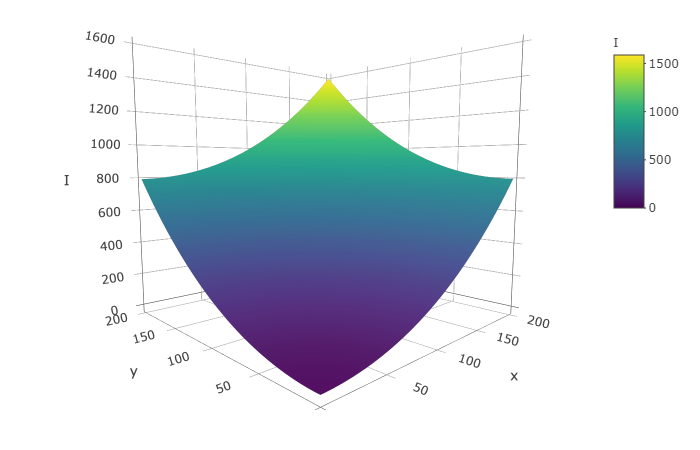
\includegraphics[width=.8\textwidth]{capitulos/figures/plot3d.png}
    \label{fig:normal}
\end{figure}

\subsubsection{Modelos Normais e de Laplace}
\label{laplace}

Assumimos desta vez que $g$ segue uma distribuição de Laplace, tal que $g(x) = \frac{1}{2}\exp(-|x|)$ e $f(x) = N(\mu, \sigma^2)$. Neste caso nós teríamos:
\begin{align*}
    E_G[\log g(X)] &= -\log 2 - \frac{1}{2}\int_{-\infty}^{\infty}|x|e^{-1|x|}dx\\
                   &= -\log 2 - \frac{1}{2}\int_{-\infty}^{\infty}xe^{-x}dx\\
                   &= -\log 2 -1,\\
    E_G[\log f(X)] &= -\frac{1}{2}\log(2\pi\sigma^2) - \frac{1}{4\sigma^2}\int_{-\infty}^{\infty}(x - \mu)^2e^{-|x|}dx\\
                   &= -\frac{1}{2}\log(2\pi\sigma^2) - \frac{1}{4\sigma^2}(4 + 2\mu^2).
\end{align*}
então, a divergência de K-L é dada por:
\begin{align*}
    I(g,f) = \frac{1}{2}\log(2\pi\sigma^2) + \frac{2 + \mu^2}{2\sigma^2} - \log 2 - 1.
\end{align*}

\begin{figure}[!h]
    \centering
    \caption{Valores da digergência de K-L para uma distribuição normal-laplace, dado $\mu = 0$}
    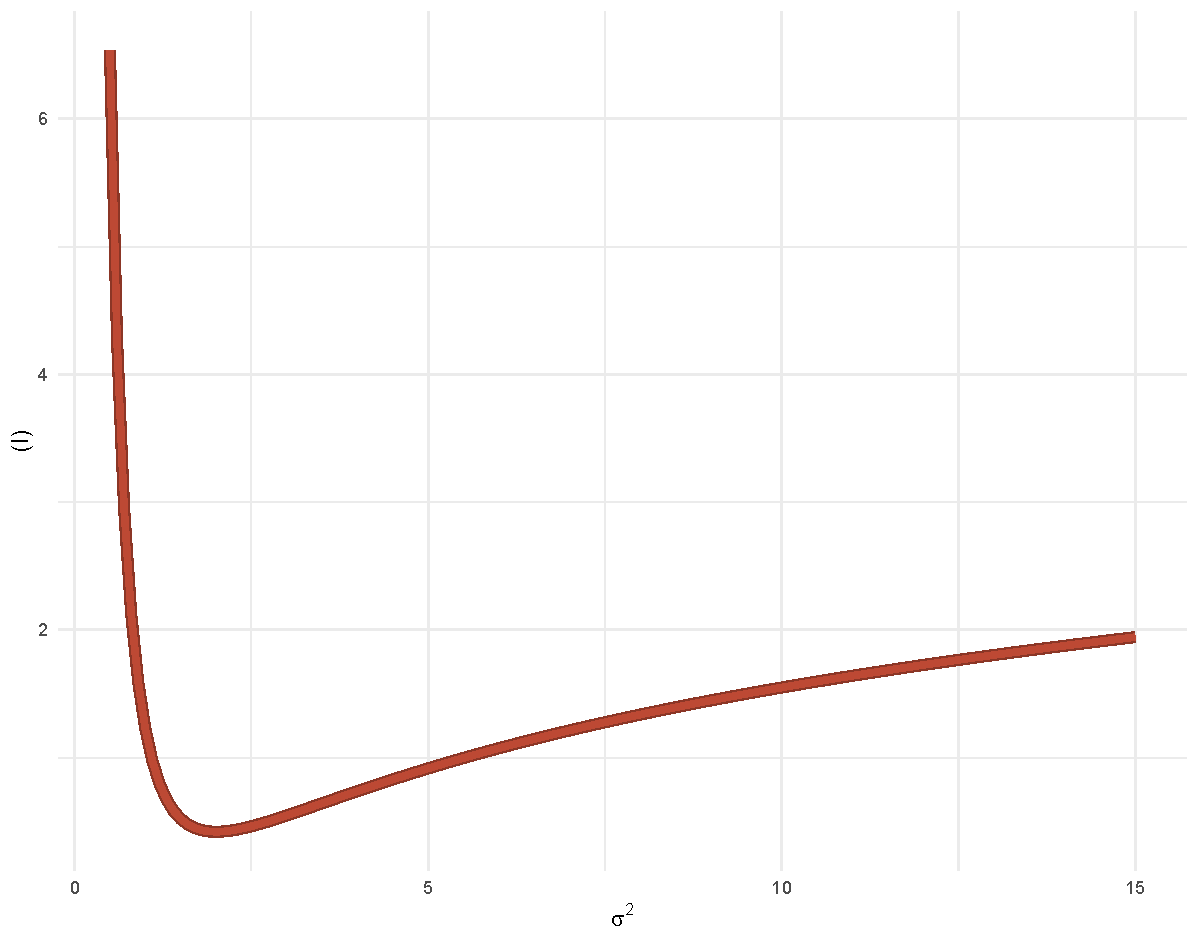
\includegraphics[width=.6\textwidth]{capitulos/figures/laplace.pdf}
    \label{fig:laplace}
\end{figure}

Em ambos os casos, podemos variar os parâmetros (nas distribuições normais, fixar $\sigma$ e permitir a variação de $\tau$ e $\Theta$, e em relação ao normal laplace, permitir a variação de $\sigma$ e $\mu$)

\section{A Análise de Sentimentos e o Índice de \textit{Otimismo}}

Analisar o que um texto expressa não necessariamente é algo simples. Automatizar este processo, além disso, pode ser algo bem custoso. A questão fundamental de uma analise de sentimentos é saber o que uma frase; texto; quer - essencialmente - expressar. Esta técnica nos permite identificar, por exemplo, a polaridade de um texto, se esse se manifesta de forma mais positiva ou negativa. É possível, além disso, contabilizar as palavras mais ditas num texto - ou num conjunto de textos, bem como suas distribuições de frequências. 

A partir do momento que possuímos um texto, precisamos tratá-lo. Existem técnicas diferentes para esse tratamento. Neste trabalho, utilizamos dicionários de \textit{stopwords}. Isso é, dado um texto qualquer, removemos \textbf{todas as palavras} contidas num dicionário de \textit{stopwords}. 

É comum que em qualquer que seja o texto, possuamos palavras que \textit{de forma geral} não contribuiriam de maneira nenhuma para entendermos o que o texto está expressando. De forma geral, dicionários de \textit{stopwords} estão em inglês - bem como os dicionários léxicos - e então somos forçados a trabalhar com textos em inglês\footnote{O COPOM disponibiliza suas atas em inglês (minutes)}. Geralmente, palavras de um dicionário de \textit{stopwords} concentram-se em palavras como ``\textit{the}'', ``\textit{and}'', ``\textit{these}'',``\textit{of}'' (tabela \ref{tab:stopwords}). Esta tabela contém exemplos de palavras de um dicionário de \textit{stopwords} disponível no pacote \textbf{tidytext} \cite{tidystop} disponível para a linguagem R. Este dicionário apresenta três dicionários léxicos de \textit{stopwords}, o \textbf{onix}; o \textbf{SMART} e o \textbf{snowball}\footnote{http://www.lextek.com/manuals/onix/stopwords1.html, http://www.jmlr.org/papers/volume5/lewis04a/lewis04a.pdf, http://snowball.tartarus.org/algorithms/english/stop.txt}. 

Neste trabalho, utilizaremos a análise de sentimentos para montarmos um índice simples de otimismo, configurado da seguinte forma \cite{costa2016ensaios}:

\begin{align} \label{indice} 
    I_O &= \frac{N_P}{N_P + N_N}
\end{align}

Isso é, em \ref{indice} representamos que o valor do índice é dado pelo número total de palavras positivas ($N_P$) dividido pela soma do número total de palavras positivas mais o número total de palavras negativas ($N_N$). Ainda, de tal forma que $0 \leq I_O \leq 1$.  
\begin{table}[!h]
\centering
\caption{Exemplos de palavras de um dicionário de \textit{stopwords}}
\begin{tabular}{lllllll}
  \hline
 a & across & all & also & and & anyway & are \\ 
 a's & actually & allow & although & another & anyways & aren't \\ 
 able & after & allows & always & any & anywhere & around \\ 
 about & afterwards & almost & am & anybody & apart & as \\ 
 above & again & alone & among & anyhow & appear & aside \\ 
 according & against & along & amongst & anyone & appreciate & ask \\ 
 accordingly & ain't & already & an & anything & appropriate & asking \\ 
   \hline
\end{tabular}
\label{tab:stopwords}
\end{table}

A classificação das palavras, é feita, entretanto, por meio de um dicionário léxico. Dicionários léxicos, na maioria das vezes, são dicionários criados por instituições de pesquisa que visam classificar palavras com valores de forma - ou não - categórica. Dessa maneira, a cada palavra é atribuído um valor ou uma característica. 

A tabela \ref{tab:lexico} apresenta palavras de um dicionário léxico proposto por Minqing Hu e Bing Liu \cite{hu2004mining} de polaridade contido no pacote \textbf{qdapDictionaries} \cite{qdapdict}, parte do \textit{software R}. Neste exemplo, o dicionário visa classificar uma palavra de forma positiva ou negativa, tal que $palavra = -1$ se negativa ou $palavra = 1$ se positiva.

\begin{table}[!h]
\centering
\caption{Exemplos de palavras de um dicionário léxico}
\begin{tabular}{rlrlrlr}
  \hline
 & \textbf{Palavra} & \textbf{Valor} & \textbf{Palavra} & \textbf{Valor} & \textbf{Palavra} & \textbf{Valor} \\ 
  \hline
1 & a plus & 1.00 & abomination & -1.00 & abrade & -1.00 \\ 
  2 & abnormal & -1.00 & abort & -1.00 & abrasive & -1.00 \\ 
  3 & abolish & -1.00 & aborted & -1.00 & abrupt & -1.00 \\ 
  4 & abominable & -1.00 & aborts & -1.00 & abruptly & -1.00 \\ 
  5 & abominably & -1.00 & abound & 1.00 & abscond & -1.00 \\ 
  6 & abominate & -1.00 & abounds & 1.00 & absence & -1.00 \\ 
   \hline
\end{tabular}
\label{tab:lexico}
\end{table}

\section{Vetor Auto-regressivo}

O surgimento dos modelos auto-regressivos são oriundos da década de 80, como alternativa às críticas dos grandes números de restrições impostas às estimações pelos modelos estruturais \citeonline{var2012bcb}. 

\begin{citacao}
``A ideia era desenvolver modelos dinâmicos com o mínimo de restrições, nos quais todas as variáveis econômicas
fossem tratadas como endógenas. Sendo assim, os modelos VAR examinam relações lineares entre cada variável e os valores defasados dela própria e de todas as demais variáveis, impondo como restrições à estrutura da economia somente: a escolha do conjunto relevante de variáveis e do número máximo de defasagens envolvidas nas relações entre elas.'' \cite[p.1]{var2012bcb}
\end{citacao}

\noindent
matematicamente, é possível representar um modelo VAR de primeira ordem (VAR(1)) da seguinte forma:
\begin{align} \label{var1}
\begin{split}
    y_{1t} &= \delta_1 + \phi_{11}y_{1,t-1} + \phi_{12}y_{2,t-1} + u_{1t} \\
    y_{2t} &= \delta_2 + \phi_{21}y_{1,t-1} + \phi_{22}y_{2,t-1} + u_{2t}
\end{split}
\end{align}

\noindent
onde $y_1$ e $y_2$ são variáveis endógenas e $u_1$ e $u_2$ são os resíduos para cada equação. $\phi_{12}$ por sua vez representa a dependência linear de $y_{11}$ em $y_{2, t-1}$ na presença de $y_{1, t-1}$ - isso é, representa o efeito condicional de $y_{2, t-1}$ sobre $r_{1t}$, dado $y_{1, t-1}$. Dessa forma, se $\phi_{12} = 0$, então $y_{1t}$ não depende de $y_{2, t-1}$. De forma análoga, se $\phi_{21}=0$, então a segunda equação mostra que $y_{2t}$ não depende de $y_{1, t-1}$ quando $y_{2, t-1}$ é dado. Ainda, podemos representar o sistema \ref{var1}, da seguinte forma:

\[
\begin{bmatrix}
    y_{1t} \\
    y_{2t}
\end{bmatrix}
=
\begin{bmatrix}
    \delta_1 \\
    \delta_2 \\
\end{bmatrix}
+
\begin{bmatrix}
    \phi_{11}y_{1,t-1} \\
    \phi_{21}y_{1,t-1} \\
\end{bmatrix}
+
\begin{bmatrix}
    \phi_{12}y_{2,t-1} \\
    \phi_{22}y_{2,t-1} \\
\end{bmatrix}
+
\begin{bmatrix}
    u_{1t} \\
    u_{2t} \\
\end{bmatrix}
\]\\

\noindent
ou, de acordo com as definições apropriadas \cite[p.322]{verbeek2008guide}:
\begin{align*}
    \Vec{Y}_t = \phi + \Theta \Vec{Y}_{t-1} + \Vec{\epsilon_t} 
\end{align*}

\noindent
onde $\Vec{Y}_t=[ y_{1t}, y_{2t}]'$ e $\Vec{\epsilon_t}=[u_{1t}, u_{2t}]'$. Isso estende um modelo auto-regressivo de primeira ordem para um caso de \textit{mais dimensões}. De forma geral, um VAR(p) para um vetor k-dimensional pode ser dado por:
\begin{align*}
    \Vec{Y}_t = \phi + \Theta_1 \Vec{Y}_{t-1} + \dots + \Theta_p \Vec{Y}_{t-p} + \Vec{\epsilon}_t
\end{align*}
\noindent
onde cada $\Theta_j$ é uma matriz $k \times k$ e $\Vec{\epsilon}_t$ é um vetor de comprimento $k$ de ruídos brancos (\textit{white noises}), com matriz de covariância $\sum$. No caso \textit{univariado}, poderíamos definir a matriz polinomial a partir do operador \textit{lag}:
\begin{align*}
    \Theta(L) = I_k - \Theta_1 L - \dots - \Theta_p L^p
\end{align*}
\noindent
sendo $I_k$ uma matriz identidade $k$. Logo, poderíamos escrever o VAR como:
\begin{align*}
    \Theta(L)\Vec{Y}_t = \phi + \Vec{\epsilon}_t.
\end{align*}
\noindent
a matriz \textit{lag} polinomial é uma matriz $k \times k$, onde cada elemento corresponde a ordem $p$ num polinômio $L$

O modelo VAR implica um modelo ARMA para cada um de seus componentes. As vantagens em se considerar os componentes de forma simultânea é que o modelo acaba por ser mais parcimonioso, inclui menos \textit{lags}, e possibilita previsões mais precisas, visto que o conjunto de informações é estendido para incluir também o histórico das outras variáveis \cite[p.322]{verbeek2008guide}. Por uma outra perspectiva, \citeonline{sims1980macroeconomics} afirma que o uso de modelos VAR ao invés de equações simultâneas estruturais é vantajoso, isso porquê a distinção entre variáveis exógenas e endógenas não tem que ser feita \textit{a priori} e de restrições `arbitrária' não são necessárias.    

\section{Função de impulso resposta} \label{respostaimpulso}

Da mesma forma que é possível representar um auto-regressivo a partir do seu componente de média móvel, podemos escrever um VAR como um vetor de média móvel (VMA). A representação de um VMA é funcionalidade essencial na metodologia de \citeonline{sims1980macroeconomics}, que permite traçarmos as diferentes projeções dado choques nas variáveis contidas no VAR. Considerando a representação matricial de um VAR(1), temos:

\begin{align} \label{var1mat}
\begin{bmatrix}
    y_{1t} \\
    y_{2t}
\end{bmatrix}
=
\begin{bmatrix}
    \delta_1 \\
    \delta_2 \\
\end{bmatrix}
+
\begin{bmatrix}
    \phi_{11}y_{1,t-1} \\
    \phi_{21}y_{1,t-1} \\
\end{bmatrix}
+
\begin{bmatrix}
    \phi_{12}y_{2,t-1} \\
    \phi_{22}y_{2,t-1} \\
\end{bmatrix}
+
\begin{bmatrix}
    u_{1t} \\
    u_{2t} \\
\end{bmatrix}    
\end{align}

\noindent
ou, podemos representar da seguinte forma:

\begin{align} \label{var1mat}
\begin{bmatrix}
    y_{1t} \\
    y_{2t}
\end{bmatrix}
=
\begin{bmatrix}
    \overline{y_1} \\
    \overline{y_2} \\
\end{bmatrix}
+ \sum_{i=0}^{\infty}
\begin{bmatrix}
    \phi_{11}y_{1,t-1} \\
    \phi_{21}y_{1,t-1} \\
\end{bmatrix}
+
\begin{bmatrix}
    \phi_{12}y_{2,t-1} \\
    \phi_{22}y_{2,t-1} \\
\end{bmatrix}
+
\begin{bmatrix}
    u_{1t} \\
    u_{2t} \\
\end{bmatrix}    
\end{align}
